% !TEX TS-program = lualatex
\documentclass[11pt]{article} 
\usepackage[margin=1in]{geometry} 
\usepackage[parfill]{parskip}% Begin paragraphs with an empty line rather than an indent
\usepackage{graphicx}
%\pdfmapfile{=newpx.map}
%\pdfcompresslevel=0
%\pdfgentounicode=1
%\input glyphtounicode.tex
%%\usepackage{pdfx} % v 1.6.4 or higher
%\InputIfFileExists{glyphtounicode-cmr.tex}{}{}
%\InputIfFileExists{glyphtounicode-ntx.tex}{}{}
\usepackage{xcolor}
\usepackage{fonttable}
\usepackage{amsmath} % must be  loaded before amsthm
\usepackage{amsthm} 
\newtheoremstyle{oldplain}
  {\topsep}   % ABOVESPACE
  {\topsep}   % BELOWSPACE
  {\itshape}  % BODYFONT
  {}       % INDENT (empty value is the same as 0pt)
  {\bfseries} % HEADFONT
  {.}         % HEADPUNCT
  {5pt plus 1pt minus 1pt} % HEADSPACE
  {}          % CUSTOM-HEAD-SPEC
\theoremstyle{oldplain}
\newtheorem{oldthm}{Theorem}[section]
\theoremstyle{plain}
\newtheorem{thm}{Theorem}[section]  
\usepackage{url}
%SetFonts
% newpx text and math
\linespread{1.05}
%\usepackage[largesc,theoremfont]{newpxtext}
\usepackage{trace}

\usepackage[theoremfont,trueslanted,scosf]{newpxtext}
\makeatletter
\ifzpl@otf
	\setmonofont{inconsolata}[Scale=MatchLowercase]
\else
	\usepackage[T1]{fontenc}
	\usepackage[scaled=.98]{zi4}
	\pdfmapfile{=newpx.map}
\fi
\makeatother

%\usepackage[scaled=1.05,zerostyle=a]{newtxtt}
\usepackage{textcomp}
\usepackage{newpxmath}
\usepackage{bm}
%\useosf
%\useproportional
%\ifzpl@lining\show\foo\else\show\barf\fi
%SetFonts
\usepackage{upquote}
\makeatletter
  \ifzpl@otf
    \def\pcf{\addfontfeatures{Letters=PetiteCaps}}
    \def\pcf{\addfontfeatures{Letters=SmallCaps}}
  \else
    \font\pcf=zpl-Regular-osf-sc-t1 at 10.95pt
    \font\scf=zpl-Regular-osf-scl-t1 at 10.95pt
  \fi
\makeatother
\DeclareMathSymbol{\Sumop}{\mathop}{largesymbols}{"50}
\usepackage{booktabs}
\title{New PX font package}
\author{Michael Sharpe}
\date{\today}  % Activate to display a given date or no date
\usepackage{scalefnt}
%\pagestyle{empty}
\begin{document}
%\show\scshape
%1\textsc{23Xx}\\
%
%\makeatletter
%{\fontfamily{zpl\zpl@figurealign OsF}
%      \fontshape\scdefault\selectfont 23Xx}
%\makeatother      
%\fonttable{zpl-Regular-osf-scl-t1}
%%\expandafter\show\csname textlf \endcsname
\maketitle
%\textcircled{R}\symbol{"00AE}{\color{red}\rule[135pt]{-3em}{.05ex}}\
%\bfseries
%\slshape
%\show\scshape
%\expandafter\show\csname scshape \endcsname
%\let\scshape\undefined
%\newfontfamily\scshape[Letters=SmallCaps,Scale=1.078]{TeXGyrePagellaX}
%2{\lfstyle2}\textlf{2}\texttlf{2}{\tlfstyle2}\textsu{2}\textde{2}\textinf{2}
%\traceon
%\textfrac[2]{7}{8}
%\traceoff
%\end{document}
%\fonttable{zpl-Regular-osf-scl-t1}
%Test\textsc{Text}{\scf Text}{\pcf Text}
%
%
%X\textsu{ABCX1234}
%{\sustyle 2}\textfractionsolidus{\destyle 5}
%
%\textfrac12 \textfrac23 \textfrac34 \textfrac45 \textfrac56  \textfrac67 \textfrac78 \textfrac89 \textfrac90 \textfrac01 %{\vrule width.04pt\char"2044\vrule width.04pt}
%%\setbox0\hbox{\zplLF\char"2044}\showthe\wd0
%%\setbox1\hbox{\char"2044\addfontfeatures{RawFeature=+ss20;+dnom}\color{red}\char"2044}\showthe\wd1
%\textcircled{M}\textcircled{2}


%\scalefont{5}{\vrule width.04pt\char"2044\vrule width.04pt}%\addfontfeatures{RawFeature=+ss20;+dnom}\color{red}\char"2044\vrule width.04pt{}4}
%{23\textsu} \textde{45} \textnu{78} \textinf{90}
%X{\sufigures 8Abc}
%\end{document}
%\show\slshape
\section{Introduction}
This package is meant to be  a replacement for Young Ryu's {\tt pxfonts}---a complete text and math package with roman text font provided by a Palatino clone, sans serif based on a \textsf{Helvetica} clone, typewriter faces, plus math symbol fonts whose math italic letters are from a Palatino Italic clone. As with the related {\tt txfonts} (though not as severe) the math metrics in {\tt pxfonts} seem overly tight.

\textsc{Changes as of version 1.53}
\begin{itemize}
\item
Superior letters and figures distinct from numerators have been added along with some special features. The text switch \verb|\sustyle| (or \verb|\sufigures|) or the commands \verb|\textsu|, \verb|\textsup|, \verb|\textsups| may be used to invoke ordinary superiors. The command \verb|\textsuperior| is reserved for a form of superiors that respond to adjustments you may specify in the package options, and which are used for footnote marker placement: \verb|supscale| rescales them, \verb|supsraised| specifies an amount to move them vertically, and \verb|supLspaced|, \verb|supRspaced| specify additional kerning to be applied at the left and right. These changes are applied in the order: scaling, raising, kerning. All except \verb|supscale| should be dimensions with units like {\tt em} which will scale properly. Their relative vertical positions stack up like this: X\textinf{12}X\textde{345}X\textnu{678}X\textsu{90}. \textbf{IMPORTANT: As of version 1.535, the options and code described in this paragraph have been moved to the new {\tt superiors} package.}
\item
Unless you specify the option {\tt defaultsups}, the package will use the superior letters and numbers for footnote markers. These will work in all LaTeX engines, and with all standard LaTeX classes, as well a the KOMA classes. With {\tt defaultsups}, you get scaled-down glyphs which may not match the color of other text and may be more difficult to find on a page.
\item
There are now characters in the superiors which may be useful in displaying symbolic footnote markers: \textsu{\textsection, \textparagraph, \textdagger, \textdaggerdbl, \textbardbl, \textasteriskcentered}. See the documentation to the {\tt footmisc} package for more details of their usage. A usage example is appended as the last page of this document.
\item Option {\tt scosf}, which specifies oldstyle figure within small caps, has been extended and now works in all LaTeX engines with both the \verb|\scshape| switch and the macro \verb|\textsc{}|.
\item
The stacked fraction macro is now available: see the documentation in the {\tt newtx} package.
\item
Version 1.53 brings {\tt newpxtext} essentially up to parity with {\tt newtxtext}, version 1.73.
\item 
Version 1.533 introduces some new mathematical glyphs. First,  there are new curly braces invoked by the option {\tt curlybraces} with {\tt height+depth} of 1.053 times 940, 1200, 1800, 2400, 3000 and 3600 em units. Second, there are three new math symbols:
\begin{itemize}
\item
\verb|\laplace|, $\laplace$, which is an inverted \verb|\nabla|, having more weight in the  bottom segment than \verb|\Delta|, $\Delta$.
\item
\verb|\laplac|, $\laplac$. This is the unicode-math name for the official d'Alembertian operator, {\tt U+29E0}. Unlike  $\laplace$, it has more weight in the left and top segments than \verb|\laplace|.
\item \verb|\dAlembertian|, $\dAlembertian$, rotates $\laplac$ by 180${}^\circ$, making for a glyph whose weight distribution is a better match for the Laplacian.
\end{itemize}
\end{itemize}
\textsc{Changes as of version 1.51}
\begin{itemize}
\item
There is a new {\tt newpx.sty} that  offers simplifications in the use of {\tt newpxtext} and {\tt newpxmath} under [pdf]latex, xelatex and lualatex. With {\tt newpx}, you can pass options to {\tt newpxtext} and {\tt newpxmath} as appropriate. For example
\begin{verbatim}
\usepackage[scale=.98,varbb,p,osf]{newpx}
\end{verbatim}
would send {\tt scale=.98} to both text and math packages, {\tt varbb} to {\tt newpxmath} and the rest to {\tt newpxtext}. Later sections have more usage examples. 
\item
{Newpxtext.sty} now has a stacked fraction macro:  \verb|\textsfrac[2]{17}{32}| produces \textsfrac[2]{17}{32}. 
\item
Version 1.51 brings {\tt newpxmath} essentially up to parity with {\tt newtxmath}, version 1.723.
\end{itemize}
\textsc{Changes as of version 1.5}\\
 {\tt newpxtext.sty} contains code that mostly works for both {\tt pdflatex} as well as {\tt XeLateX} and {\tt LuaLaTeX}, though there are some new features that work only with the last two. The precise differences will be spelled out below. Unless explicitly noted, macros and package options will function similarly for all LaTeX engines.
%The goal of this new project is use his glyphs along with a few additions and with completely reworked metrics which are generally looser, but not as loose as Computer Modern math. The following small examples (double normal size) provide some idea of the  extent of the changes.


%\begin{minipage}{3.1in}
%\begin{center}
%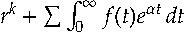
\includegraphics[scale=2]{pxfontseg-crop}\\
%Math rendered with pxfonts
%\end{center}
%\end{minipage}
%\begin{minipage}{3.1in}
%\begin{center}
%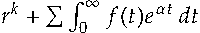
\includegraphics[scale=2]{newpxeg-crop}\\
%Math rendered with newpxmath
%\end{center}
%
%\end{minipage}


The original {\tt newpx} package differed from {\tt pxfonts} in the following ways, all of which are preserved in the newest version:
\begin{itemize}
\item
{\tt newpx} is split into separate text and math packages that do not need to be used in conjunction;
\item both text and math packages offer options not present in the original package, described below;
\item wide accent glyphs have been corrected (they should have zero depth) so that they no longer collide with the underlying glyph;
\item the summation and product symbols in {\tt pxfonts} seemed overly heavy at display size, and have been replaced by others of more suitable weights;
\item for those who do not like the integral in \textsf{pxfonts}, an emboldened version of the Computer Modern integral is made available, matching the weight of the \textsf{pxfonts} symbols;
\item an upright partial derivative symbol has been added, named \verb|\uppartial|---$\uppartial$;
\item 
braces and other delimiters are now larger and, I believe, more pleasing to older eyes;
\item macros have been added to bring the calls to Greek symbols more into conformity with \textsc{psnfss} and Mathtime Pro~2;
\item an upright Greek \verb|\upvarkappa|, $\upvarkappa$, has been added as well as a matching italic version $\varkappa$;
\item problems using \textsc{ams} macro packages before \textsf{pxfonts} are settled;
\item \verb|\coloneq| and \verb|\eqcolon| now point to the correct glyphs;
\item The problem with the {\tt ogonek} accent  and tabular environments (bad definition of \verb|\k|) is fixed;
\item The default encoding for \textsf{newpxtext} is now T$1$, but support is offered also for OT$1$ and LY$1$. As some add-on packages are available only in T$1$, that seems the best current choice.
\item The font collection used for rendering text is based on TeXGyrePagella with a number of additions, named TeXGyrePagellaX. The superior figures in this addition are set by default to render footnote markers. (It is also possible customize footnote markers by redefining \verb|\thefootnote| after loading {\tt newpxtext.sty}.) 
\item Sans serif is by default taken from TeXGyreHeros, a Helvetica clone, and by default at 94\% of the scale factor (set by {\tt scaled}, default value {\tt1}). The option {\tt helvratio=.98} will change that to 98\%. As of newpx version 1.415, there is an option {\tt nohelv} that prevents this loading.
\item New math accents such as \verb|\widearc| have been introduced in tandem with the {\tt newtx} package, where they are documented.
\end{itemize}


\section{Text mode options and macros}

\textsc{Important changes as of version 1.5}
\begin{itemize}
\item
 Small caps are available in all weights and styles, and are offered in two sizes. The default small caps supplied by TeXGyrePagella are really {\pcf Petite Caps}, having xheights approximately the same x-heights (sometimes smaller) as lowercase letters. Option \texttt{largesc} increases the size of small caps by  5.33\%, approximating the size of Linotype Palatino Small Caps. IMO, this is a better match in terms of weight and size: {\pcf Petite Caps}, \textsc{Small Caps}. The two sizes of small caps are now implemented in the Opentype fonts as Petite Caps and Small Caps ({\tt pcap} and {\tt smcp}). The option {\tt largesc} changes the default rendering of \verb|\scshape| and \verb|\textsc| to Small Caps instead of the default Petite Caps. 
 
\item The last versions were missing the switches \verb|\tlfstyle|,  \verb|\lfstyle|, \verb|\tosfstyle| and \verb|\osfstyle| as well as their command forms  \verb|\texttlf|,  \verb|\textlf|, \verb|\texttosf| and  \verb|\textosf|, which allowed you to get any figure alignment and style, no matter what the default figure style. For example, though  the main text is proportional oldstyle, \verb|\texttlf{123}| gives the tabular lining form \texttlf{123}, as does \verb|{\tlfstyle123}|.

\item There are also the commands \verb|\oldstylenums|, \verb|\liningnums|, \verb|\tabularnums| and \verb|\proportionalnums|, which change only the alignment and the style.

\item Two additional figure styles have been added---denominators and subscripts (inferiors), each the same size as superiors, with denominators having the same baseline as text and subscripts below the text baseline.  These may be specified  respectively by the text switches \verb|\defigures| (\textsc{aka} \verb|\destyle|) and \verb|\infigures| (\textsc{aka} \verb|\instyle|) or the corresponding macros \verb|\textde| and  \verb|\textinf|. For example, \verb|{\defigures 123}| gives {\defigures 123}, as would \verb|\textde{123}|, and  \verb|{\infigures 123}| gives {\infigures 123}, as would \verb|\textinf{123}| or \verb|\textsub{123}|.
\item There is a numerators figure style normally used only in the construction of fractions. It may be called by any one of \verb|{\nustyle 123}|, \verb|{\nufigures 123}|, \verb|\textnum{123}|, \verb|\textnumerator{123}|. There is also an equivalent named \verb|\textnu{123}|, but this is problematic since it conflicts with a command in the Greek variant of the {\tt babel} package. If you use the latter, there is an option {\tt notextnu} to {\tt newtxtext} that will prevent the redefinition of \verb|\textnu|.
\item There is a new version of \verb|\textfrac| that provides better kerning around the division solidus than the default command. The integer part may be specified as an optional argument. E.g., \verb|\textfrac{7}{8}| gives \textfrac{7}{8}, while \verb|\textfrac[2]{31}{32}| gives \textfrac[2]{31}{32}.

\item There is a new \verb|\textcircled| which works with both letters and numbers.\\
 E.g., \verb|\textcircled{X}\textcircled{2}| gives \textcircled{X}\textcircled{2}.
\item A new option {\tt slashedzero} is provided for XeLaTeX and LuaLaTeX only. It replaces the zero in lining style only to a zero with a reverse slash.
\end{itemize}

\textsc{Important changes as of version 1.42}\\
Option  {\tt theoremfont} was reimplemented using a new font family, {\tt npxth} instead of abusing \verb|\textsl|. By default,  users of {\tt theoremfont} will see no change in its functionality, including the use of the macro \verb|\textsl| to output italics with upright punctuation. A new option, {\tt trueslanted}, to {\tt newpxtext} has the following effects:
\begin{itemize}
\item
\verb|\textsl| now outputs slanted text rather than italics with upright punctuation text, but not affecting the usage of the {\tt theoremfont} option to {\tt newpxtext}.
\item the former behavior of \verb|\textsl| is now available through the new macro \verb|\textth|, \textsc{aka} \verb|\textthit|.
\item \verb|\pagestyle{headings}| now functions as originally intended with slanted rather than upright figures in the headers.
\end{itemize}

The text mode environment invoked by
\begin{verbatim}
\usepackage{newpxtext}
\end{verbatim}
has several options: you may write
\begin{verbatim}
\usepackage[scaled=.95]{newpxtext}
\end{verbatim}
to load the roman and typewriter text fonts at 95\% of normal size, and the sans serif (\textsf{Helvetica} clone) at scale 0.95\textasteriskcentered0.94. This is not of much utility if the package is used with the math package {\tt newpxmath} to which it is already matched, but may be with other math packages. The options
\begin{verbatim}
\usepackage[scaled=.95,helvratio=.96]{newpxtext}
\end{verbatim}
load roman and typewriter text fonts at 95\% of normal size, and the sans serif (\textsf{Helvetica} clone) at scale 0.95*0.96.

The option \texttt{osf} instructs the text fonts to use old-style figures \oldstylenums{1234567890} rather than the default lining figures \texttlf{1234567890}. As of version 1.23, {\tt newpxtext} loads initially with lining figures so the math package uses lining figures in math mode. The option {\tt osf} switches to old-style figures in text at the very end of the preamble, forcing the use of oldstyle figures in text, but not math. In previous versions, it was necessary to run 
\verb|\useosf| after loading math. This is no longer required, but does no harm. See the discussion in section 4 for further details. A similar macro \verb|\useproportional| makes proportional figures the default outside math mode. 

As of version 1.415, the new option {\tt nohelv} prevents the loading of the default Helvetica clone as the sans serif text font. If you use this option, you should load your preferred sans serif font, otherwise you will be left with the Computer Modern default.

As described above, option {\tt largesc} increases the size of small caps by  5.33\% so that the height matches that of the small caps in Linotype Palatino.

Option {\tt defaultsups} (same effect as {\tt defaultsups=true}) forces the package to use the \LaTeX\ default footnote markers (or, at least, those in force when the package is loaded) instead of those preferred by the package---Palatino (clone) superior figures instead of spindly ordinary Palatino lining figures reduced to about 70\%. (Footnote markers in minipages use the default lowercase alphabetic characters, unless otherwise specified by redefining \verb|\thempfootnote|.) For better control over position and size of footnote markers, use the {\tt superiors} package after loading {\tt newpxtext}. 

The {\tt theoremfont} option changes the default font used for the {\tt plain} theorem style of {\tt amsthm}, keeping italic text but substituting upright figures and punctuation. For example, with this option, you get theorem statements like this:

\begin{thm}
This is Theorem Italic: text numbers are upright---12345; punctuation is in many cases upright (also, parens (), braces \{\} and brackets []). What about question marks and exclamations? Also upright! [These fit better with math mode punctuation and figures, like: for all $x\in[0,1]$, let $f(x)\coloneq \exp(\alpha x)$].
\end{thm}
Compare this to traditional {\tt plain} theorem style of the same text:
\begin{oldthm}
This is Theorem Italic: text numbers are upright---12345; punctuation is in many cases upright (also, parens, braces \{\} and brackets []). What about question marks and exclamations? Also upright! [These fit better with math mode punctuation and figures, like: for all $x\in[0,1]$, let $f(x)\coloneq \exp(\alpha x)$].
\end{oldthm}

If you are using another theorem package (e.g., ntheorem, theorem) you will have to add your own descriptors as specified in the its documentation and set the body font to \verb|\thfamily|.

Superior letters and figures may be called with either \verb|{\sustyle ...}| or \verb|\textsu{...}|, so you can emulate $18$\textsu{th} century orthography such as J\textsu{os} W\textsu{m} Smith, or print French style with , e.g., $1$\textsu{i\`ere}, M\textsu{me} Dubois or M\textsu{lle} D'Orl\'eans.

The next two sections describe options to {\tt newpxtext} of more specialized nature.

\section{Spacing issues}%\footnote{The options described in this section are different under XeLaTeX and LuaLaTeX.}
This new version of {\tt newpxtext} has spacing that is a little different, in its default state, from that of the old {\tt newpxtext}. In small part this is due to the finer kerning of TeXGyre Pagella, but mostly because the three parameters that govern inter-word spacing are not the same.
\begin{verbatim}
                               pxfonts     Pagella
fontdimen2 (interword space)   .25em       .25em
fontdimen3 (interword stretch) .125em      .2em
fontdimen4 (interword shrink)  .08333em    .1em
\end{verbatim}
That is, {\tt Pagella} has the same normal spacing as {\tt pxfonts} but its spacing is more flexible in terms of both stretch and shrink. More frequently than not, a paragraph built with {\tt Pagella} will occupy more space than the same built with {\tt pxfonts}. For this reason, the package offers some ways to change the spacing parameters. This may be important if you are trying to imitate the pagination of a document built using~{\tt pxfonts}.

\textbf{Behavior under [pdf]LaTeX.}\\
Option {\tt tighter} sets the three fontdimen values to those of {\tt pxfonts}, except with a little more shrink. This should make it unlikely that text will occupy more space than it would have using~{\tt pxfonts}. 

Option {\tt looser} sets the three fontdimen values to \verb|{.3em,.2em,.1em}| respectively. 

If you want full control, the options {\tt spacing, stretch, shrink} allow you to modify one or more of the above fontdimens. For example,
\begin{verbatim}
\usepackage[stretch=.15em,shrink=.095em]{newpxtext}
\end{verbatim}
\textbf{Behavior under XeLaTeX and LuaLaTeX.}\\
Fontspec  offers the {\tt WordSpace=} option for individual control of the space, stretch and shrink, with the value being either an ordered triple like \verb|{1.1,1,.8}| or a single number like {\tt .9}, the latter having the same effect as the triple \verb|{.9,.9,.9}|. These three numbers act as multipliers of {\tt space}, {\tt stretch} and {\tt shrink}. The option that you can set is {\tt spcfactor=}, entering either a number or a triple---e.g., {\tt spcfactor=1.1} or \verb|{1.1,1,.8}|. Note however that {\tt tighter} and {\tt looser} will have an effect if {\tt spcfactor} is not set, amounting to \verb|{\spcfactor={1,.625,1}| and \verb|{\spcfactor={1.2,1,1}| respectively.

\subsection{Basic example preambles.}

The examples below are unrealistically simple but do show the structure of the part of the preamble required to load {\tt newpx}.

\textsc{I: Otf text, otf math (requires unicode engine)}


Supports an arbitrary otf math font with otf text using {\tt TeXGyreTermesX}.
\begin{verbatim}
	% Without newpx package:
    \usepackage[otfmath]{newpxtext}
    \usepackage{unicode-math} %loads amsmath
    \setmathfont{}[]  %expects your input here for otf math font and options
% or, with newpx package:
    \usepackage[otfmath]{newpx} % pass options to text package
    \setmathfont{}[]  %expects your input here for otf math font and options
\end{verbatim}
\textsc{Notes:}
\begin{itemize}
\item Your option list to {\tt newpx[text]} must include {\tt otfmath}, otherwise it will load {\tt newpxmath}. 
\item With {\tt newpx}, you may specify certain other otf text fonts.
\item After loading {\tt newpx}, you must load your chosen unicode math package with \verb|\setmathfont{}[]|.
\item
You do not need to load {\tt amsmath}: it is loaded by {\tt unicode-math}.
\item When using an otf math font, options to {\tt newpx} are passed only to {\tt newpxtext}.

\item Babel, if used, must be specified before {\tt newpx[text]}, which loads {\tt fontspec}.
\item Polyglossia, if used, must be specified after loading {\tt newpx[text]}.
\end{itemize}

\textsc{II: Otf text, type1 math (requires unicode engine)}

Supports  {\tt newpxmath} with an otf text font.
\begin{verbatim}
% Without newpx
    \usepackage[T1]{fontenc} % so operators can have accented letters
    \usepackage[list of math options]{newpxmath} % loads minimal version of text font for use in math 
    \usepackage[no-math]{fontspec}
    \usepackage{} % the chosen otf text font package, or fontspec \setmainfont, etc
% or, using newpx, only for TeXGyrePagellaX
    \usepackage[T1]{fontenc} % so operators can have accented letters
    \usepackage[list of text and math options]{newpx} 
    % options will be passed to text font package and newpxmath
\end{verbatim}
\textsc{Notes:}
\begin{itemize}
\item No special option requirements---this is the default case.
\item You may load sans and tt text fonts before {\tt newpx} if you wish \verb|\mathsf| and \verb|\mathsf| not to be the default {\tt helvetica} and {\tt cmtt}.
\item Babel, if used, must be specified before {\tt newpx[text]}, which loads {\tt fontspec}.
\item Polyglossia, if used, must be specified after loading {\tt newpx[text]}.
\end{itemize}



\textsc{III: type1 text, type1 math (requires non-unicode engine)}

In the olden days  of [pdf]latex processing, {\tt newpx} was traditionally summoned with lines like
\begin{verbatim}
\usepackage[T1]{fontenc}
\usepackage[<list of text options>]{newpxtext}
\usepackage[<list of math options>]{newpxmath}
\end{verbatim}
which still works but is a bit less flexible than its modern form:
\begin{verbatim}
\renewcommand*{\rmdefault}{min
zpltlf}% minimal text family, Roman and Bold for math
\usepackage[T1]{fontenc}
\usepackage[<list of text and math options>]{newpx}
\end{verbatim}
which expands in the non-unicode case to
\begin{verbatim}
\renewcommand*{\rmdefault}{minzpl}
% minimal text family, Roman and Bold for math
\usepackage[T1]{fontenc}
\usepackage[<list of math options>]{newpxmath}
\usepackage[<list of text options>]{newpxtext}
\end{verbatim}
For this arrangement, the math package needs information about the text font currently in force and the current typewriter and, possibly, the current sans serif font. The default Latin Modern text family would most likely not work well here for use as operators, \verb|\mathbf|, \verb|\mathtt| and the like. Dealing with the math part first allows you the flexibility of choosing different text fonts  for use in math than you will use for body text.
\begin{verbatim}
% Without newpx
    \renewcommand*{\rmdefault}{minzpl}% minimal text family, Roman and Bold for math
    \usepackage[T1]{fontenc}
    \usepackage[<list of math options>]{newpxmath} % options will be as passed from newpx
    \usepackage{} % the chosen text package
    % should load tt and sans math before math
% or, using newpx, where text font will be TeXGyrePagellaX
    % should load tt and sans math before newpx
    \usepackage[T1]{fontenc} % math text font zpltlf by default
    \usepackage[<list of text and math options>]{newpx} 
\end{verbatim}
\textsc{Notes:}
\begin{itemize}
\item Babel, if used, must be specified before {\tt newpx[text]}.
\end{itemize}

Note that with a unicode engine, it is not possible to load a type1 text font package unless you have created custom {\tt tu}-encoded support files.

\section{Usage with {\tt babel}}
You should normally load {\tt babel} before loading {\tt newpxtext} in order for {\tt babel} to function as expected.  For example, using {\tt pdflatex}:
\begin{verbatim}
\usepackage[greek.polutonico,english]{babel}
% the next line makes text figures proportional, oldstyle, while math uses lining figures
\usepackage[theoremfont,trueslanted,largesc,tighter,p,osf]{newpxtext}
\usepackage[T1]{fontenc}
\usepackage{textcomp}
\usepackage[varqu,varl]{inconsolata}
\usepackage{amsmath} % must be loaded before amsthm, if using amsthm
\usepackage{amsthm} % must be loaded before newpxmath
\usepackage[vvarbb]{newpxmath}
% option vvarbb gives you stix blackboard bold
\linespread{1.05}
\end{verbatim}
With {\tt newpx}, you could simplify this a bit.
\begin{verbatim}
\usepackage[greek.polutonico,english]{babel}
\usepackage[varqu,varl]{inconsolata}
\usepackage[T1]{fontenc}
% the next line makes text figures proportional, oldstyle, while math uses lining figures
\usepackage[theoremfont,trueslanted,largesc,tighter,p,osf,amsthm,vvarbb]{newpx}
% amsmath is loaded automatically, before amsthm
% option vvarbb gives you stix blackboard bold
\linespread{1.05}
\end{verbatim}
 
\section{Usage with Lua\LaTeX\ and Xe\LaTeX}
As far as I can tell, \textsf{newpxmath} works with both, but requires a very specific loading order and choice of options. Briefly,  the math options must all be loaded prior to loading and using {\tt fontspec}. As of version 1.5, {\tt newpxtext} will load {\tt fontspec} when processing with XeLaTeX or LuaLaTeX unless one  option {\tt type1} is specified. (Option {\tt nofontspec} is no longer acted upon, having no proper function, as of version 1.506.) If you specify the option {\tt no-math} to {\tt newpxtext}, it will pass that option to the {\tt fontspec} call. This should be specified if  {\tt fontspec} will not be expected to load an Opentype math font.

\textsc{Example I: TeXGyrePagellaX Opentype + texgyrepagella-math (Opentype).}
\begin{verbatim}
%\usepackage[greek.polutonico,english]{babel} % if using babel
% next line calls fontspec and loads TeXGyrePagellaX otf
\usepackage[otfmath,theoremfont,trueslanted,largesc,p,osf]{newpxtext}
% set mono and sans opentype fonts
%\usepackage{polyglossia} % must load after fontspec, if using polyglossia
% polyglossia setup commands
\usepackage{unicode-math}% can't load type1 math fonts after this
\setmathfont{texgyrepagella-math}
%  \mathsf and \mathtt from Latin Modern
% operators and other \mathxx from TeXGyrePagellaX
\end{verbatim}
\textsc{Notes:}
\begin{itemize}
\item
You do not need to load {\tt amsmath}: it is loaded by {\tt unicode-math}.
\item Babel, if used, must be specified before {\tt newpxtext}, which loads {\tt fontspec}.
\item Polyglossia, if used, must be specified after loading {\tt newpxtext}.
\end{itemize}
With {\tt newpx}, there is a little simplification:
\begin{verbatim}
%\usepackage[greek.polutonico,english]{babel} % if using babel
% next line calls fontspec and loads TeXGyrePagellaX otf
\usepackage[otfmath,theoremfont,trueslanted,largesc,p,osf]{newpx}
% set mono and sans opentype fonts
%\usepackage{polyglossia} % must load after fontspec, if using polyglossia
% polyglossia setup commands
%\usepackage{unicode-math}% newpx loads unicode-math
\setmathfont{texgyrepagella-math}
\end{verbatim}

%\textsc{Example II: newpxtext type1 + texgyrepagella-math (Opentype).}
%\begin{verbatim}
%%\usepackage[greek.polutonico,english]{babel} % if using babel
%% next line does not call fontspec, loads newpxtext type1 
%\usepackage[type1,theoremfont,trueslanted,largesc,p,osf]{newpxtext}
%\usepackage{fontspec}
%%\usepackage{polyglossia} % must load after fontspec, if using polyglossia
%% polyglossia setup commands
%\usepackage{unicode-math}% can't load type1 math fonts after this
%\setmathfont{texgyrepagella-math}
%\end{verbatim}
%\textsc{Notes:}
%\begin{itemize}
%\item The {\tt type1} option to {\tt newpxtext} prevents the package loading {\tt fontspec} so you must load it before loading {\tt unicode-math} and any opentype fonts.
%\item
%You do not need to load {\tt amsmath}: it is loaded by {\tt unicode-math}.
%\item Babel, if used, must be specified before {\tt newpxtext}.
%\item Polyglossia, if used, must be specified after loading {\tt fontspec}.
%\end{itemize}

\textsc{Example II: TeXGyrePagellaX Opentype + newpxmath (type1) + polyglossia + other Opentype.}
\begin{verbatim}
\renewcommand{\rmdefault}{minzpl}% Roman and Bold PagellaX for math mode
\usepackage[T1]{fontenc} % T1 is active encoding for use in math text
\usepackage[type1]{sourcesanspro}% used only by \mathsf, optional
% Next line loads amsmath, then loads amsthm
\usepackage[amsthm,vvarbb]{newpxmath}
\usepackage[no-math]{newpxtext}% pass no-math option to fontspec
% Fontspec will be loaded so that Opentype text fonts may be loaded
% By default, TeXGyrePagellaX (otf) will be loaded
%\usepackage{polyglossia} % must load after fontspec
%\setdefaultlanguage[variant=american]{english}
%\setotherlanguages{french,russian}
%\newfontfamily{\cyrillicfont}[Scale=MatchLowercase]{cochineal}
\end{verbatim}
\textsc{Notes:}
\begin{itemize}
\item The {\tt no-math} option to {\tt newpxtext} causes {\tt fontspec} to load with option {\tt no-math}, preventing the package from loading any unicode math font.
\item
You do not need to load {\tt amsmath}: it is loaded by {\tt newpxmath}. Option {\tt amsthm} will cause {\tt amsmath} to load before {\tt amsthm}.
\item Babel, if used, must be specified before {\tt newpxtext}.
\item Polyglossia, if used, must be specified after loading {\tt newpxtext}.
\item The {\tt type1} option to {\tt cabin} is important, preventing it from loading {\tt fontspec}, which would lead to an {\tt option clash} error. 
\end{itemize}
With {\tt newpx}, the above is equivalent to:
\begin{verbatim}
\usepackage[T1]{fontenc} % T1 is active encoding for use in math text
\usepackage[type1]{sourcesanspro}% used only by \mathsf, optional
% Next line loads amsmath, then loads amsthm
\usepackage[no-math,amsthm,vvarbb]{newpx}
% Fontspec will be loaded so that Opentype text fonts may be loaded
% By default, TeXGyrePagellaX (otf) will be loaded
\usepackage{polyglossia} % must load after fontspec
\setdefaultlanguage[variant=american]{english}
\setotherlanguages{french,russian}
\newfontfamily{\cyrillicfont}[Scale=MatchLowercase]{cochineal}
\end{verbatim}

\textsc{Example III: newpxtext type1 + newpxmath (type1) + polyglossia + other Opentype.}
\begin{verbatim}
\renewcommand{\rmdefault}{minzpl}% Roman and Bold Pagella for math mode
\usepackage[T1]{fontenc} % T1 is active encoding for use in math text
\usepackage[type1]{sourcesanspro}% used only by \mathsf, optional
%Uncomment either the following line
%\usepackage[amsthm,vvarbb,no-math]{newpx}
%or the next pair of lines
%\usepackage[amsthm,vvarbb]{newpxmath}
%\usepackage[no-math]{newpxtext}% pass no-math option to fontspec

% Other Opentype text fonts may be loaded here
\usepackage{polyglossia} % must load after fontspec
\setdefaultlanguage[variant=american]{english}
\setotherlanguages{french,russian}
\newfontfamily{\cyrillicfont}[Scale=MatchLowercase]{cochineal}
\end{verbatim}
\textsc{Notes:}
\begin{itemize}
\item
You do not need to load {\tt amsmath}: it is loaded by {\tt unicode-math}.
\item Babel, if used, must be specified before {\tt newpxtext}.
\item Polyglossia, if used, must be specified after loading {\tt newpx [text]}.
\end{itemize}

%\textsc{Example V: newpxtext tfm + texgyrepagella-math.}

Be aware that some text packages (e.g., {\tt cabin}) may contain a line like
\begin{verbatim}
\RequirePackage{fontspec}
\end{verbatim}
which would provoke an ``option clash'' error with  a subsequent 
\begin{verbatim}
\usepackage[no-math]{fontspec}
\end{verbatim}
unless suppressed by an appropriate option. E.g., 
\begin{verbatim}
\usepackage[type1]{cabin}
\end{verbatim}
prevents the problem with the {\tt cabin} package. (Not working in the version of {\tt cabin.sty} dated 12/25/2022. This has been corrected in the version dated 2023-09-25.)

\iffalse
 Consider three scenarios for using some part of {\tt newpx} with one of XeLaTeX, LuaLaTeX.
\subsection{Use {\tt newpxtext} and {\tt newpxmath} with {\tt fontspec} for other text fonts}
\begin{verbatim}
%load LaTeX text components before math
\usepackage[T1]{fontenc} % affects only \mathrm, \mathbf etc
\usepackage{newpxtext}
\usepackage[scaled=.85]{beramono}% used only by \mathtt, optional
\usepackage[type1]{sourcesanspro}% used only by \mathsf, optional
\usepackage[amsthm,vvarbb]{newpxmath}
\usepackage[scr=rsfso]{mathalpha} % optional
\usepackage{bm}% load after all math to give access to bold math, optional
%Now load the otf text fonts using fontspec---won't affect math
\usepackage[no-math]{fontspec} % process with XeLaTeX or LuaLaTeX
\setmainfont{TeXGyrePagellaX} % this reads in TeXGyrePagellaX.fontspec
\end{verbatim}

While the math font options must be specified before {\tt fontspec}, be aware of a potential trap. Using \verb|\usepackage{newpxtext}| before \verb|\usepackage{newpxmath}| results in {\tt newpxtext}'s font-loading options being run after all other packages in the preamble, so instead of \verb|\usepackage{newpxtext}|, do the following:

\textsc{Example:}
\begin{verbatim}
%load LaTeX text components before math
\usepackage[T1]{fontenc} % affects only \mathrm, \mathbf etc
\renewcommand{\rmdefault}{minzpl}
% Roman font for use in math mode
\usepackage[scaled=.85]{beramono}% used only by \mathtt, optional
\usepackage[type1]{sourcesanspro}% used only by \mathsf, optional
\usepackage{amsmath} % must be loaded before amsthm
\usepackage{amsthm}% load before newpxmath
\usepackage[vvarbb]{newpxmath}
\usepackage[scr=rsfso]{mathalpha} % optional
\usepackage{bm}% load after all math to give access to bold math, optional
%Now load the otf text fonts using fontspec---won't affect math
\usepackage[no-math]{fontspec} % process with XeLaTeX or LuaLaTeX
\setmainfont{TeXGyrePagellaX} % this reads in TeXGyrePagellaX.fontspec
\end{verbatim}

\textsc{Example preamble using polyglossia:}

\begin{verbatim}
\renewcommand{\rmdefault}{zpltlf}% Roman and Bold for use in math mode
\usepackage[T1]{fontenc} % T1 is active encoding for use in math text
\usepackage[type1]{sourcesanspro}% used only by \mathsf, optional
%\usepackage{amsmath} % must be loaded before amsthm
%\usepackage{amsthm}% load before newpxmath
\usepackage[amsthm,vvarbb]{newpxmath}
\usepackage[no-math]{newpxtext}% pass no-math option to fontspec
% Fontspec will be loaded so that Opentype text fonts may be loaded
\usepackage{polyglossia} % must load after fontspec
\setdefaultlanguage[variant=american]{english}
\setotherlanguages{french,russian}
\newfontfamily{\cyrillicfont}[Scale=MatchLowercase]{Cochineal}
\end{verbatim}
\fi

Previous to version 1.5, the preceding pages of this document were processed using {\tt pdflatex}, which was the only engine supported by {\tt newpxtext.sty}. As of version 1.5, XeLaTeX and LuaLaTeX are also supported and the entire document is now processes by LuaLaTeX. All {\tt newpxtext} options and macros formerly limited to {\tt pdflatex} have been modified and now work essentially the same under both unicode engines, though the output may not always be precisely the same as with {\tt pdflatex}. There are some macros and options available under unicode engines that go beyond what can be done under {\tt pdflatex}.

\textsc{Modified Macros and Options:}
\begin{itemize}
\item
\verb|\textfrac| works more precisely under unicode tex because it is possible to adjust kerning between all characters. The effect should not be very noticeable, at least in regular style. 
%\item {\tt sups}:  the package treats this differently in unicode LaTeX and pdflatex, with handling in the unicode case passed off to the {\tt realscripts} package where the footnote marker font is set to \verb|\normalfont|, meaning that superiors from the current (TeXGyrePagellaX) text font are employed.
%\item The \verb|\footnote| macro has been changed and appears to function correctly in KOMA based packages, though for proper handling of multiple footnote markers it may be necessary to add the following line to your preamble:
\begin{verbatim}
\usepackage[multiple]{fontmisc}
\end{verbatim}
\item {\tt theoremfont}, {\tt thmtabular}, {\tt thmlining} all function in a manner similar to that in {\tt pdflatex}.
\item {\tt swashQ} operates as before.
\item {\tt foresolidus, aftsolidus} are not used in unicode tex.
%\item {\tt scosf} operates more effectively than in [pdf]latex---in the latter, it seems now very difficult to modify the definition of \verb|\scshape|, and this option works only for \verb|\textsc|.
%you have the choice of font to render footnote markers. The differences are as follows.
%\begin{itemize}
%\item
%{\bfseries Unicode latex:}
%\begin{itemize}
%\item
%if you include the option {\tt sups} to {\tt cochineal} and there is no {\tt fnmarkerfont=} option set, then  footnote markers are taken from the Cochineal-Roman superiors.
%\item if there is a {\tt fnmarkerfont=} option set, then, whether or not there iss a {\tt sups} option set, then, if available, footnote markers will be taken from the superiors in the font family that {\tt fnmarkerfont=} is set to. (When trying a font family, try this in your preamble:
%\begin{verbatim}
%\newfontfamily\mysu{EBGaramond}{\addfontfeatures{RawFeature=+sups}}
%\end{verbatim}
%and then, in the body of your document, try typesetting
%\begin{verbatim}
%X{\mysu 123}X 
%\end{verbatim}

%\end{itemize}
%\item
%{\bfseries pdflatex:}
%\end{itemize}•
%if you do not include the {\tt fnmarkerfont=} option but you do include {\tt sups}, then footnote markers are taken from {\tt Cochineal-Roman-sups}. There is a new option, {\tt fnmarkerfont} that you can use to specify the font to use for footnote markers. It is ignored when using {\tt pdflatex}.
\item \verb|\textcircled| works the same as under {\tt pdflatex}.%\textcircled{X}\textcircled{2}
\end{itemize}
\textsc{New Macros and Options:}
\begin{itemize}
%\item
%An alternate version of Q, 
%\Qswash\space (\verb|\Qswash|) and their small cap versions is available using option {\tt altQ}, which sets {\tt StylisticSet=3}. The alternate versions are {\addfontfeatures{RawFeature=+ss03}Q}, {\addfontfeatures{Style=Swash,RawFeature=+ss03}Q}.
%\item
%An alternate version of J is available in italic shapes only using option {\tt altJ}, which sets {\tt StylisticSet=2}. The alternate version of \textit{J} is {\itshape {\addfontfeatures{RawFeature=+ss02}\textit{J}}}.
%%.\textit{J} {\textbf{Bold}} \textsc{SmallCap}
\item {\tt oldSS} controls whether the new German capital sharp S is used or whether the old SS is retained. The former is the default but the option {\tt oldSS} forces the latter by setting {\tt StylisticSet=6}. The effects are summarized in the following tables.
\makeatletter
\ifzpl@otf
\makeatother

\begin{center}
  \begin{tabular}{@{} lcl @{}}
    \hline
    Glyph name & glyph & macro\\ 
    \hline
    {\tt uni1E9E} & \symbol{"1E9E} &\verb|\symbol{"1E9E}| or \verb|\SS|\\ 
    {\tt uni1E9E.ss06} & {\addfontfeature{StylisticSet=6}\symbol{"1E9E}} & \verb|{\addfontfeature{StylisticSet=6}\symbol{"1E9E}}| \\ 
    {\tt germandbls.sc} & \textsc{\ss} & \verb|{\textsc{\ss}}| \\ 
    {\tt germandbls.sc.ss06} & {\addfontfeature{StylisticSet=6,RawFeature=+smcp}\ss} & \verb|{\addfontfeature{StylisticSet=6}\textsc{\ss}}| \\ 
    \hline
  \end{tabular}
\end{center}  
\fi % \ifzpl@otf
\end{itemize}
%{\bfseries
%\begin{center}
%  \begin{tabular}{@{} lcl @{}}
%    \hline
%    Glyph name & glyph & macro\\ 
%    \hline
%    {\tt uni1E9E} & \symbol{"1E9E} &\verb|\symbol{"1E9E}|\\ 
%    {\tt uni1E9E.alt} & {\addfontfeature{StylisticSet=1}\symbol{"1E9E}} & \verb|{\addfontfeature{StylisticSet=1}\symbol{"1E9E}}| \\ 
%    {\tt germandbls.sc.ss01} & {\addfontfeature{StylisticSet=1}\textsc{\ss}} & \verb|{\addfontfeature{StylisticSet=1}\textsc{\ss}}| \\ 
%    \hline
%  \end{tabular}
%\end{center}
%}
 \noindent Effect of choice of {\tt StylisticSet}:
\makeatletter
\ifzpl@otf
\makeatother
 
\begin{center}
  \begin{tabular}{@{} ccccc @{}}
    \hline
    StylisticSet & \verb|\ss| & \verb|\SS| & \verb|\MakeUppercase{\ss}| & \verb|\textsc{\ss}| \\ 
    \hline
    None & \ss & \SS & \MakeUppercase{\ss} & \textsc{\ss}\\ 
    
    =6 & {\addfontfeature{StylisticSet=6}\ss} & {\addfontfeature{StylisticSet=6}\SS} & {\addfontfeature{StylisticSet=6}\MakeUppercase{\ss}} & {\addfontfeature{StylisticSet=6}\textsc{\ss}}\\ 
    \hline
  \end{tabular}
\end{center}
\fi % \ifzpl@otf

\section{Math mode options}
The package invoked by
\begin{verbatim}
\usepackage{newpxmath}
\end{verbatim}
loads the math part of the {\tt pxfonts} (with revised metrics and additional glyphs) and should be loaded \emph{after} the text font and its encoding have been specified, as it uses the text font settings to define how operators, numbers, math accents, \verb|\mathrm|, \verb|\mathbf| etc.\ are rendered. You should also load a Typewriter font so as not to generate mysterious error messages about \textsf{metafont} trying to generate \texttt{ectt10}. The package offers a number of options.
\begin{itemize}
\item {\tt upint} (new as of version 1.3.) selects upright integrals---the default shape is slanted. Each shape/size of integral takes one of twelve form, illustrated below in the case of display size slanted integrals.
\[\int\quad\oint\quad\iint\quad\iiint\quad\iiiint\quad\oiint\quad\oiiint\quad\varointclockwise\quad\ointctrclockwise\quad\fint\quad\sumint\quad\sqint\]
named respectively
\begin{verbatim}
\int \oint \iint \iiint \iiiint \oiint 
\oiiint \varointclockwise \ointctrclockwise \fint \sumint \sqint
\end{verbatim}
The three sizes of the upright integrals look like:
\begin{center}
  \begin{tabular}{@{} cl @{}}
    \hline
    Glyph & Command\\ 
    \hline
    $\smallintup$ & \verb|\smallint[up]|\\ 
    $\intup$ & \verb|\int[up]|  \\ 
    $\displaystyle{\intup}$ & \verb|\displaystyle{\int[up]}|\\ 
    \hline
  \end{tabular}
\end{center}
Note that the suffix {\tt up} is not required unless the document's integral style is slanted. You may find the \verb|\smallint| is useful for inline math mode when it is important not to change the line spacing.
\item {\tt smallerops} (new as of version 1.3.) causes big operators other than integrals to render up to 20\% less tall, so that displayed formulas may occupy less vertical space. For example, in the following display, the first operator is the usual \verb|\sum|, the second is what you would get with {\tt smallerops}, the third is \verb|\textstyle{\sum}| and the fourth is \verb|\smallsum|, the latter being used mainly with inline math. 
\[\sum \Sumop \textstyle{\sum} \smallsum\]
Similarly, there are \verb|\smallprod| and \verb|\smallcoprod| which, along with \verb|\smallsum|, are of class {\tt mathop}, unlike their Greek letter equivalents.
\item (New as of version 1.3.) Two macros allow you to change {\tt fontdimen} values in math mode: \verb|\setSYdimens| and \verb|\setEXdimens|, which allow you to change the {\tt fontdimen} parameters for the {\tt symbol} and {\tt extension} fonts respectively. They may be used only in your preamble. Their arguments can be any valid \TeX\ commands to change {\tt fontdimen} values. For example:
\begin{verbatim}
\def\setSYdimens{\fontdimen16\font=2pt\fontdimen17\font=1.15\fontdimen17\font }
\end{verbatim}
Don't use these unless you know what you're doing.
\item 
\begin{itemize}
\item{\tt varg} causes the math italic letter $g$ to be replaced by $\varg$;
\item{\tt cmintegrals} instructs \textsf{newpxmath} to load a thicker version of the Computer Modern integral in place of the \textsf{newpxmath} default---the pxfonts integral (identical to the integral in the Wolfram fonts), which is not to everyone's taste---a consequence is that none of the special forms of \textsf{pxfonts} integrals are available; \textbf{As of version 1.3, this option does nothing, as the new default is slanted integrals.}
\item The former option {\tt cmbraces} instructed {\tt newpxmath} to ignore the brace collections from {\tt pxfonts}, substituting a collection based on thickened versions of the Computer Modern braces, which I found much easier to distinguish from other delimiters. This worked quite well in regular weight but looked a bit clunky in bold. It no longer has any effect.
\item The once new option {\tt bigdelims} offered delimiters which were a bit larger than the standard delimiters and the normal and {\tt big} sizes, with more distinction between the two than in the standard package. With {\tt bigdelims}, the option {\tt cmbraces} was ignored. Now, {\tt bigdelims} is the default, and the option has no effect.
\end{itemize}
\item the combination
\begin{verbatim}
\usepackage{amsmath}% loads amstext, amsbsy, amsopn but not amssymb
\usepackage{newpxmath}
\end{verbatim}
causes no error, unlike the same combination with {\tt pxfonts}, but does nothing significant. The package {\tt newpxmath} loads the package {\tt amsmath} if it was not previously loaded. Options to {\tt amsmath} such as {\tt leqno,intlimits} may be passed to {\tt amsmath} via options to the documentclass. 
%The integrals are as defined in {\tt pxfonts}. %With
%\begin{verbatim}
%\usepackage[cmintegrals]{newpxmath}
%\end{verbatim}
%you may use the forms \verb|\iint|, \verb|\iiint|, \verb|\iiiint| and \verb|\idotsint| defined in {\tt amsmath}, but using the pumped-up Computer Modern integral loaded by {\tt newpxmath}. 
\item {\tt uprightGreek} and {\tt slantedGreek} determine the form of Greek alphabet loaded---the default is {\tt uprightGreek}, which loads upright uppercase and slanted lowercase Greek symbols, as is customary in Anglo-American mathematical typesetting. With the option {\tt slantedGreek}, which you might want to use if you cared about ISO standards, all Greek symbols are slanted. No matter which is set, \verb|\Gammaup| (or \verb|\upGamma|) gives you upright \verb|\Gamma|, etc, and \verb|\Deltait|, \verb|zetait| give you italic (i.e., slanted) versions of those letters, and \verb|\mathnormal{\Omega}| etc will always produce the slanted version of uppercase Greek letters. (The macro \verb|\mathnormal| means essentially ``use the version of the symbol in {\tt letters}''---i.e., the math italic form. This did not always work as expected in versions prior to 1.27.)
\item The \textsf{newpxmath} package contains three different Blackboard Bold alphabets, where original \textsf{pxfonts} contained one. The default, triggered by \verb|\mathbb{}|, takes its glyphs from the font which replaces {\tt msbm} and has the same overall appearance of a hollowed-out text font, which I find neither bold nor blackboard-like. The second option, taken from \textsf{pxfonts}, is triggered by \verb|\varmathbb{}|, is more geometric and, in my opinion, preferable but not optimal. The option {\tt varbb} makes \verb|\mathbb{}| synonymous with \verb|\varmathbb{}|. The third option is the double-struck glyphs from the STIX collection. See the expanded discussion below.
\item {\tt nosymbolsc} causes the package to not load the {\tt symbolsC} fonts, saving  a math family. (This font contains mostly exotic symbols, along with some very useful, commonly used symbols like \verb|\coloneq| $\coloneq$, \verb|\eqcolon| $\eqcolon$, \verb|\notin| $\notin$, \verb|\notni| $\notni$, \verb|\neq| $\neq$, \verb|\nsubset| $\nsubset$ and \verb|\nsupset| $\nsupset$, but these have been moved (virtually) to {\tt lettersA} so they may continue to be used even if you use the option {\tt nosymbolsc}.)
\item {\tt amssymbols} (the default) and {\tt noamssymbols} determine whether the {\tt pxfonts} versions of the \textsc{ams} symbols ({\tt msam}, {\tt msbm}) are loaded---if so, they override previous settings in {\tt amsmath}. If you use the option {\tt noamssymbols}, then \verb|\mathbb{}| is set to mean the same as \verb|\varmathbb{}|. (One advantage of {\tt noamssymbols} is that you save one of your precious math families for other purposes, such as setting a couple of external math alphabets by means of the \textsf{mathalfa} package.)
\end{itemize}

\textsc{Example:}
\begin{verbatim}
\documentclass[leqno]{article}
\usepackage[osf,theoremfont]{newpxtext} % T1, lining figures in math, osf in text
\usepackage{textcomp} % required for special glyphs
\usepackage[varg]{newpxmath} % single story g
\usepackage[scr=rsfso]{mathalpha}% \mathscr is fancier than \mathcal
\usepackage{bm} % load after all math to give access to bold math
%\useosf %no longer needed unless using babel
\linespread{1.05}% Give Palatino more leading (space between lines)
\end{verbatim}

\section{Some recent additions to \texttt{newpxmath}}
Because a number of the standard math accents appeared to be too close to the symbols they accented, a number of the problem accents have been reworked as additions to the {\tt symbols} font, along with a number of vertically doubled symbols. (The doubled symbols are described in the documentation to newtx.) The new accents are flatter and stand higher above their accentees than the old versions.

Another addition to {\tt symbols} may be used to signify matrix \emph{transpose}. In fact, the glyph is just the {\tt intercal} glyph (from the txfonts rendition of the AMS symbols) raised and narrowed considerably. Here is an example comparing its use to a number of other common constructions:
\[\mathbf{M}^{\transp}, \mathbf{M}^{\mathsf{T}}, \mathbf{M}^{\mathrm{T}}, \mathbf{M}^{\intercal},\]
are produced respectively by
\begin{verbatim}
\mathbf{M}^{\transp}, \mathbf{M}^{\mathsf{T}}, \mathbf{M}^{\mathrm{T}},
 \mathbf{M}^{\intercal}.
\end{verbatim}
Clearly, the last needs to have the exponent raised and moved to the left. This is not hard to do, but it may use up on of your math families unless you are already using the AMS symbols. A similar objection could be made to the use of \verb|\mathsf|.
\section{The \TeX\ math font problem}
Math font packages in \LaTeX\ are susceptible to the ``Too many math alphabets'' error, due to exceeding the limit of just sixteen math font families, or mathgroups, as they are called in \LaTeX. Put in oversimplified terms that do however correctly represent how this all works in \textsf{newpxmath}, the following math fonts are always loaded and permanently (if you didn't prevent loading of some features) occupying slots immediately following \verb|\begin{document}|, and others that may be called for in typesetting a mathematical expression can add to the list as the document grows.

\textsc{Always loaded:}
\begin{verbatim}
0: operators
1: letters
2: symbols
3: largesymbols
4: AMSm (replaces former AMSa and AMSb)
5: lettersA
6: symbolsC
7: largesymbolsTXA
8: boldoperators
9: boldletters
10: boldsymbols
11: boldlargesymbols
\end{verbatim}
\textsc{Notes:}
\begin{itemize}
\item
The {\tt operators} font is essentially the Roman text font, used for names of operators and as the target for \verb|\mathrm|---its bold version is used as the target for \verb|\mathbf|;
\item if you typeset an expression that, say, calls for a single bold glyph from  {\tt symbolsC}, that costs you an entire new slot, leaving only two remaining;
\item same with, e.g., \verb|\mathit|;
\item same with an external Fraktur, Blackboard Bold or Script glyphs;
\item if you run out of math alphabets, look first to dropping {\tt AMSm} and  {\tt symbolsC}, which can save you at least two slots;
\item if space is tight, do not call bold versions of the fonts listed above where the bold version is not already loaded, to avoid loading a new mathgroup; 
\item if you absolutely need a letter (not a math symbol) from some math font that would normally cost you another mathgroup, you might consider using as if it were text, with something like
\begin{verbatim}
\mbox{{\usefont{U}{zplmia}{b}{n} X}}
\end{verbatim}
which allows you to use letter X from {\tt boldlettersA} but without any math features;
\item there is a macro \verb|\ShowMathFonts| in {\tt newpxmath} which may be called at any point in your document, which will provide you a list of the mathgroups currently in use. This can be helpful in figuring out where problems occur. The output lines take the form
\begin{verbatim}
(<fam number>: <internal font id> = <tfm name> [newpx name])
\end{verbatim}

\end{itemize}
\section{Bold math fonts}\label{sec:boldmath}
Every math font in the {\tt pxfonts} package, and in the {\tt newpx} package, is accompanied by a bold version. Some usage examples are given below. Generally, one may use either \verb|\boldmath| to change an entire formula to bold, or \verb|\boldsymbol| to change one symbol, but the spacing generally works better after loading the {\tt bm} package and using the \verb|\bm| macro.

The text glyphs dotlessi (\verb|\i|) and dotlessj (\verb|\j|) are rarely needed in actual text---in many fonts, roman dotlessi is very similar to the numeral 1. They are however sometimes needed to build special math glyphs. The following table shows how to generate the mathematical forms of dotlessi and dotlessj. I illustrate with only dotlessi---dotlessj is entirely analogous.

\begin{center}
  \begin{tabular}{@{} llll @{}}
    \hline
    Type & Weight & Command & Result \\ 
    \hline
    Math Italic & Regular & \verb|$\hat{\imath}$| & $\hat{\imath}$ \\ 
    Math Italic & Bold & \verb|$\bm{\hat{\imath}}$| & $\bm{\hat{\imath}}$ \\ 
    Roman & Regular & \verb|$\hat{\textrm{\i}}$| & $\hat{\textrm{\i}}$\\ 
    Roman & Bold & \verb|$\bm{\hat{\textbf{\i}}}$| & $\bm{\hat{\textbf{\i}}}$\\ 
    \hline
  \end{tabular}
\end{center}
\newcommand{\xyvec}[2]{\ensuremath{#1\bm{\textbf{\i}}#2\bm{\textbf{\j}}}}

In math, bold roman characters are often used to indicate vector quantities, and for this one uses constructions like 
\begin{itemize}
\item
\verb|$\mathbf{x}$| produces $\mathbf{x}$;
\item
\verb|$\bm{\mathrm{x}}$| produces $\bm{\mathrm{x}}$ (same as previous but may offer improved spacing);
\item
\verb|$\bm{x}$| produces $\bm{x}$ (not roman);
\item
\verb|$\bm{\hat{\mathbf{x}}}$| produces $\bm{\hat{\mathbf{x}}}$ (with a bold accent);
\item \verb|$\bm{\dot{x}}$| produces $\bm{\dot{x}}$ (bold but not roman);
\item the macro definition
\begin{verbatim}
\newcommand{\xyvec}[2]{\ensuremath{#1\bm{\textbf{\i}}#2\bm{\textbf{\j}}}}
\end{verbatim}
allows you to write \verb|\xyvec{x}{+y}| to output $\xyvec{x}{+y}$;
\item \verb|$\bm{\Gamma}$| produces $\bm{\Gamma}$ (bold Gamma);
\item \verb|$\bm{\hat{\Gamma}}$| produces $\bm{\hat{\Gamma}}$ (bold Gamma with bold accent).
\end{itemize}
(The last two assume that you have effectively set the option {\tt uprightGreek}---the default.)

\section{Blackboard bold}
As mentioned briefly above, the package now has a new blackboard bold alphabet built-in, and some new macros to call the non-default versions. To summarize, the problems are:
\begin{itemize}
\item
the default, called by \verb|\mathbb| is quite ugly and indistinct, but does cooperate with the bolding macros \verb|\bm| and \verb|\boldsymbol|;
\item the original variant form called with the macro \verb|\varmathbb| is better, but the macro conflicts with \verb|\bm|. (In fact, the bold version is identical to the regular version, but it is still not right that it conflicts with them.) The problem stems from the part of the definition of \verb|\varmathbb| which allows you to insert an argument with more than one character, like \verb|\varmathbb{ABC}|. The solution is to make a new macro that takes a single argument, like \verb|\vmathbb{A}|, which cooperates with \verb|\bm|.
\item the third, new, alphabet is borrowed from the STIX fonts---it is sharp and quite clear, geometric in design. The macro \verb|\vvmathbb| provided to access this alphabet allows only a single character for its argument. The new option {\tt vvarbb} effectively makes \verb|\mathbb| mean the same as \verb|\vvmathbb|.
(The reason for including these in the \textsf{newpx} package rather than calling them from the \textsf{mathalfa} package is that \textsf{newpx} leaves very little space for new math symbol fonts and math alphabets, and this way requires no additional such resources.
\end{itemize}
One interesting feature of the new alphabet is that it contains blackboard bold numbers, of which $0$ and $1$ will likely be the most useful, perhaps as operator names. I find $\vvmathbb{1}$=\verb|$\vvmathbb{1}$| useful in specifying an indicator, AKA characteristic function. Here are some examples:

\begin{center}
  \begin{tabular}{@{} llll @{}}
    \toprule
     & Regular & Bold & Remarks \\ 
    \midrule
Default  & \verb|$\mathbb{R}$| $\mathbb{R}$& \verb|$\bm{\mathbb{R}}$| $\bm{\mathbb{R}}$\\ 
Variant 1     & \verb|$\varmathbb{R}$| $\varmathbb{R}$ &  & Bold is same as regular \\ 
$\dots$or     & \verb|$\vmathbb{R}$| $\vmathbb{R}$ &  & Single char.\ argument\\ 
Variant 2 & \verb|$\vvmathbb{R}}$| $\vvmathbb{R}$& \verb|{\boldmath $\vvmathbb{R}$}| {\boldmath $\vvmathbb{R}$} & Make a macro for this! \\ 
%     & $\bm{\mathbb{AB}}$  & $\bm{\vmathbb{A}\vmathbb{B}}$ & $\bm{\vvmathbb{A}\vvmathbb{B}}$ \\ 
    \bottomrule
  \end{tabular}
\end{center}

For further information on the changes made to \texttt{newpxmath} 1.3, see the appendix to the documentation for \texttt{newtxmath} 1.5.

\def\jj{\mkern-3mu j}

\section{Appendix 1: Changes made in version 1.40}
Versions of {\tt newpx}  dated from September, 2019 (1.40 for {\tt newpxmath} make some quite substantial changes, mostly to math mode. 

\section{Goals}
Spurred by work of Ross Moore to provide means of generating archivable pdf using {\tt pdflatex}, the main goal was to change {\tt newpx} and {\tt newtx} to meet the requirements for satisfying the {\tt PDF/A-1b} standards by using an appropriate preamble involving the {\tt pdfx} package and other unicode mapping files. Making these  changes  gave me the opportunity to organize the source files to make them more manageable in  future revisions. 

A further goal whose time seemed ripe was to rework the  spacing of math letters, both Roman and Greek, so they behaved better in superscripts and subscripts. This did not turn out to be so easy. The problem is illustrated by math italic j. If you don't give it enough extra space on the left, it will likely collide with the D in rendering \verb|$D^j$|. On the other hand, if you do give it enough space on the left, it will look bad as a  subscript, appearing too far right. 

A final goal was to make better use of the remaining space in some of the math fonts by placing some math alphabets in them, avoiding perhaps a waste of those precious sixteen math families.

\section{The important changes}
The following changes were made to both {\tt newtx} and {\tt newpx}.

\subsection{Archivability}
Some of the individual font files from which the math fonts are built turned out to have some fairly minor structural issues. These have all been corrected. The more major issue was the lack of unicode mapping for all characters in the fonts. For the symbol and math extension fonts, this issue was largely solved by Ross Moore's {\tt glyphtounicode} files that are now accessible as part of TeXLive and MiKTeX. The main problem was the math alphabets like math italic, bold math italic, upright Greek and slanted Greek, all of which have now been assigned their own unicode points. For all of these, I constructed new fonts using unicode names for the glyphs, then made \textsf{fontinst} scripts that renamed those unicode values to the original simple names as used in the encoding files so that I could use my old encoding and adjustment files. This exercise has now been carried out for {\tt newtxmath}, {\tt newpxmath}, {\tt newtxmath/libertine} and {\tt newtxmath/xcharter.} Each of these can now be considered to have an ``enhanced'' status that allows them to share all the new assets described below. The other packages which may be specified as an option to {\tt newtxmath} (e.g., {\tt  baskervaldx}) must be considered for the moment to be ``unenhanced'' and able to share only some of the new assets. In particular, only the enhanced items can generate archivable pdf. 

Also modified were the {\tt sups} fonts in {newpxtext}, where the main issue was unicode mapping. Superior number and some superior letters do have assigned unicode values, but in may cases a more creative approach was needed, and provided once again by Ross Moore. I rebuilt the superior font files using those unicode names, solving that particular problem.

Here is a sample  preamble showing the elements you will need to specify to generate a pdf satisfying the PDF/A-1b standards, as verified by Adobe Acrobat Pro. (Other verification processes may yield different outcomes.)
\begin{verbatim}
\documentclass[noamsfonts]{amsart} % save 2 math families 
\pdfcompresslevel=0 
\pdfgentounicode=1 
\input glyphtounicode.tex 
\usepackage{pdfx} % v 1.6.4 or higher
\InputIfFileExists{glyphtounicode-cmr.tex}{}{} 
\InputIfFileExists{glyphtounicode-ntx.tex}{}{}
\usepackage{newpxtext} %T1 is default encoding
\usepackage[scaled=0.95]{inconsolata}  % typewriter
%\usepackage[leqno]{amsmath} 
\usepackage{amsmath} % must be loaded before amsthm
\usepackage{amsthm}
\usepackage[vvarbb]{newpxmath} % vvarbb gives STIX Bbb
\end{verbatim}

Version 1.6.3 of {\tt pdfx} from February 2019  mishandles math accents. A fix is now available and will become part of the upcoming {\tt pdfx} v1.6.4.

\subsection{Glyph spacing changes} I reworked the math italics to improve the rendering of some  superscripts. This affects (a)  parentheses, brackets and braces to inhibit clashes; (b) glyphs like j, f, p, y, \verb|\rho|,  \verb|\beta| and  \verb|\mu| where a long tail could pose problems intersecting with other glyphs; (c) glyphs like such as D, Q and \verb|\Phi| that are round on the right, where interference is most likely to occur with a superscript. Increasing the left side-bearing of j, etc., helps with superscripts but creates an ugly gap when used as subscripts.  


 The {\tt subscriptcorrection} option to {\tt newpxmath} has been corrected and enhanced  so that it now offers a partial solution the subscript spacing problem. I regret that this option is incompatible with xy-pic, both depending on redefining \verb|_| as an active character. {\tt Newpxmath}  will detect if the {\tt xy} package is loaded and disable {\tt subscriptcorrection} if so. You would have to correct such issues by manually inserting a negative \verb|\mkern|. For example, you might put in your preamble something like
 \begin{verbatim}
\def\jj{\mkern-3mu j}
\end{verbatim}
and then use \verb|$x_{\jj}$| instead of \verb|$x_j$|, turning $x_j$ into $x_{\jj}$.

If you do enable {\tt subscriptcorrection}, there is a default correction table in the {\tt sty} file, but the sty file also looks for a file named,  {\tt newpx-subs.tex}. There is already such a file located in the {\tt newpx} distribution in the \verb|tex/latex/newpx| folder. (The contents of this file are also listed at the end of this appendix, from which they may be more easily copied.) If you wish to make changes to this file, copy the file to your home TeX folder where it will be found by TeX before the one in the distribution. (The contents of this file are also listed at the end of this appendix, from which they may be more easily copied.) The entries in the file are lines like
\begin{verbatim}
{j}{-3}
\end{verbatim}
each of which will have the same effect as the above macro if the first item in the subscript is {\tt j}. You can also specify Greek letters with lines like
\begin{verbatim}
{\beta}{-1.5}
\end{verbatim}

\subsection{New glyphs added}  Math family 1 {\tt (letters)} has been extended from 128 slots to 256, retaining the {\tt OML} encoding of the first 128. Most of additional slots have been allocated to a script font from the old STIX collection and an upright modification of that font.
By default, \verb|$\mathscr{F}$| will produce $\mathscr{F}$.\\
$\bullet$ option {\tt uprightscript} changes the output to {\usefont{OML}{ntxmi}{m}{it}\char201}.\\
In both cases, there are full upper-case and lower-case and {\tt dotlessi}, {\tt dotlessj}. To insert the latter, you can write either \verb|$\mathscr{\imath}$| or \verb|$\imathscr$|, rendered as $\mathscr{\imath}$ in the slanted script case.

The secondary letters font {\tt (lettersA)} and math family 2 {\tt(symbols)} have been rearranged. The first of these continues to have a Fraktur alphabet, but it a modification of its original one, having wider vertical stems and a blacker appearance more in keeping with the weight Times. {\tt Dotlessi} and {\tt dotlessj} have been added and can be specified in math mode by \verb|$\imathfrak$| and \verb|$\jmathfrak$|. Note that \verb|$\mathfrak{\imath}$| also works. There are in addition two subsidiary Bbb alphabets in {\tt lettersA}, specified by the respective options {\tt vmathbb}, {\tt vvmathbb}, and there are corresponding {\tt dotlessi}, {\tt dotlessj} activated by \verb|$\imathbb$|, \verb|$\jmathbb$|, which always render as $\imathbb$, $\jmathbb$ no matter the choice of which Blackboard Bold Alphabet. If you select one of the options {\tt vmathbb}, {\tt vvmathbb}, you will have Bbb digits 0..9 using, e.g., \verb|$\mathbb{1}$| to get~$\varmathbb{1}$. (Without one of these options in force, \verb|$\mathbb{1}$| will render as~$\mathbb{1}$ because the default Bbb has no figure glyphs in the default slots.)

Among the new symbols added are:\\
$\bullet$ \verb|\hslash|, \verb|\hbar|, \verb|\lambdaslash|, \verb|\lambdabar|, \verb|\Zbar|, \verb|\Angstrom| are now constructed from the native glyphs.\\
$\bullet$ Euler's constant \verb|$\Euler$| ($\Euler$).\\
$\bullet$ Hermitian transpose \verb|\hermtransp| or \verb|\htransp| is used like \verb|$\mathbf{A}^{\htransp}$| ($\mathbf{A}^{\htransp}$). This usage is similar to simple transpose \verb|$\mathbf{A}^{\transp}$| ($\mathbf{A}^{\transp}$).\\
$\bullet$ Independence can use \verb|\Perp|, $\Perp$, and there is a new \verb|\nPerp|, $\nPerp$, for its negation.

\subsection{Adaptive vector accent} The \LaTeX\ macro \verb|\overrightarrow| provides a right arrow with adaptive width, but not matching the vector head of {\tt newpxmath}. Likewise, the {\tt esvect} provides a similar service with a choice of vector heads, none of which match {\tt newpxmath}. I've added code to provide a matching adaptive vector accent and which uses the same macro name, \verb|\vv|, as {\tt esvect}.
For a comparison of these vector accents, \verb|$\vec{XY} \vv{XY} \overrightarrow{XY}$| renders as\\ 
$\vec{XY} \vv{XY} \overrightarrow{XY}$.\\ 
$\bullet$ \verb|$\vv{AB}$|  renders as $\vv{AB}$.\\ 
$\bullet$ \verb|$\vv*{AB}{x}$| renders as $\vv*{AB}{x}$. This provides better horizontal spacing of subscripts than \verb|$\vv{AB}_{x}$|, $\vv{AB}_{x}$.\\
$\bullet$  You can also do \verb|$\vv*{AB}{\vv{CD}}$|, which  renders as $\vv*{AB}{\vv{CD}}$.\\
$\bullet$ You can change the vertical space between the arrow and the accentee by means of the package option {\tt vecsep}, whose default value is {\tt .25ex}.

\subsection{Miscellaneous Changes}
\begin{itemize}
\item
The superior letters fonts in {\tt newpx} 
have been extended and all glyphs now have appropriate unicode mappings.
\item
The AMS fonts replacement, {\tt zplsym} corrects the former misplacement of \verb|\kbbb|, \verb|\daleth|, \verb|\circledR| and \verb|\circledS|.)
\end{itemize}
\newpage
\section{Changed Font Tables}
\subsection{letters}
\fonttable{zplmi}

Note that either of the script P glyphs  in the above table would be suitable for rendering \verb|\powerset|, though this is not a standard math macro.
\newpage  
\subsection{lettersA}
\fonttable{zplmia}
\newpage  
\subsection{symbols}
\fonttable{zplsy}
\newpage 
\subsection{A sample newpx-subs.tex}
You may either copy the entire block below, starting with the line \verb|\begin{...| and ending after the line beginning \verb|\end{|
and pasting it into the top of your document before the \verb|\documentclass...| line, which will allow for easy editing and will write the file to the same folder as your document, or make your own file, omitting those outer two lines.

\begin{verbatim}
\begin{filecontents*}{newpx-subs.tex}
{f}{-2.5}
{j}{-1.5}
{p}{-1}
{y}{-1}
{A}{-1.5}
{B}{-1}
{D}{-1}
{H}{-1}
{I}{-1}
{K}{-1}
{L}{-1}
{M}{-1}
{N}{-0.5}
{P}{-1}
{X}{-1}
{\rho}{-1.5}
{\mu}{-1}
\end{filecontents*}
\end{verbatim}

%\section{Footnote markers}
%The following page displays some of the ways that footnote markers may be modified.
%\newpage
%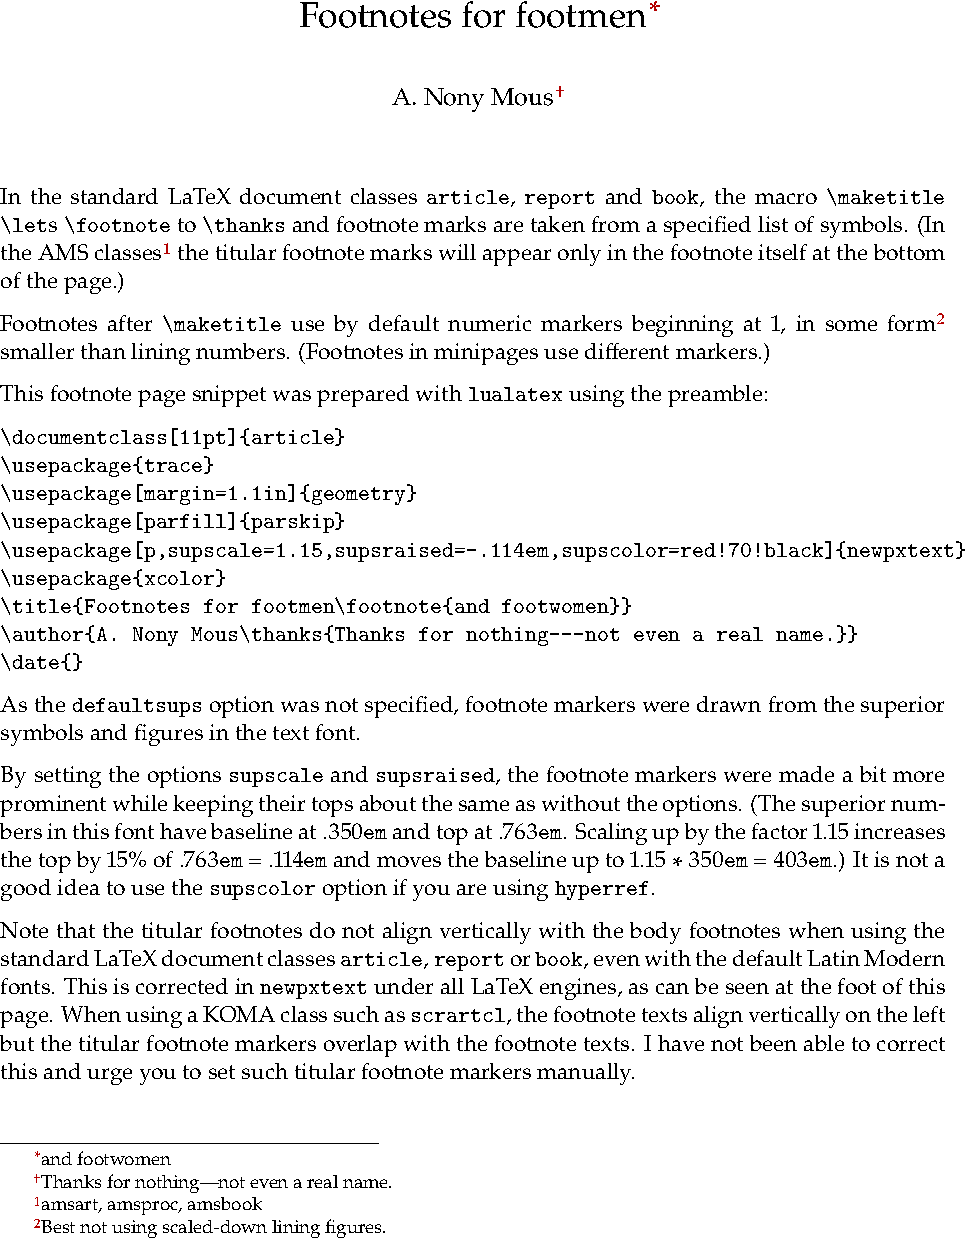
\includegraphics{footsnippet-crop}
\end{document} 
